\documentclass[]{scrartcl}

%opening
\title{March Madness}
\author{Alexander Van Roijen, Rocco Bavuso, Molly Clark}

\usepackage[margin=1.0in]{geometry}
\usepackage{color}
\usepackage{times}
\usepackage[pdftex]{hyperref}

\newcommand{\fillin}[1]{\textcolor{red}{\textsc{#1}}}

\pagestyle{empty}
\setlength{\parindent}{0in}
\setlength{\parskip}{2ex}
\renewcommand{\baselinestretch}{1.0}

\usepackage{graphicx}
\usepackage{caption}
\usepackage{float}

\begin{document}

\maketitle

\begin{abstract}
This report analyzes what it takes to become a March Madness Champion. We are taking a look at data from the past, and at winners from the past to see if there is anything specific that points to a team winning the tournament.
\end{abstract}

\section*{Introduction}
Throughout this report, we will analyze past data on March Madness teams, their seasons, and their performance in the tournament. We have gathered data from kaggle.com and broken it down to find the most useful predictors of a team winning the tournament.
\section*{Data Summary}
On Kaggle's website, we found data that gave us a look at the teams who qualified for the March Madness tournament. Each team is assigned a four digit code that is consistent from season to season in each data set. This allows us to easily manipulate and analyze the data.

We begin by looking at the data that has been collected season to season.

We follow up by looking at the data from previous tournaments to see which factors effect a team's chances of winning.
\subsection*{Regular Season Data}
Part of our analysis comes from detailed regular season data of 71,241 NCAA divison 1 games from 2003 to 2016. The data available are game statistics of winning and losing teams, such as field goals made, rebounds, assists, etc. For this part of the analysis we wanted to determine particular characteristics of winning teams in the regular season visible on the stat sheet. This part was used to help determine what are the best predictors of a winning team. In order to do so, we thought the ideal comparison would be winning team statistics compared to average team statistics. We computed this difference for the following statistics: field goal, three point, and free throw percentage, rebounds, assists, turnovers, steals, personal fouls, and blocks. The first three statistics are percentages while the rest are averages per game.  
\section*{Pre-Analysis}
\subsection*{A History Of Success}
As we all know from our sporting careers, certain teams we have watched, played against, or played with can have a history of success. Meaning, despite the ups and downs of each team from year to year, some teams are known to succeed. The same goes with college basketball, there are top performers.
\begin{figure}[H]
	\centering
	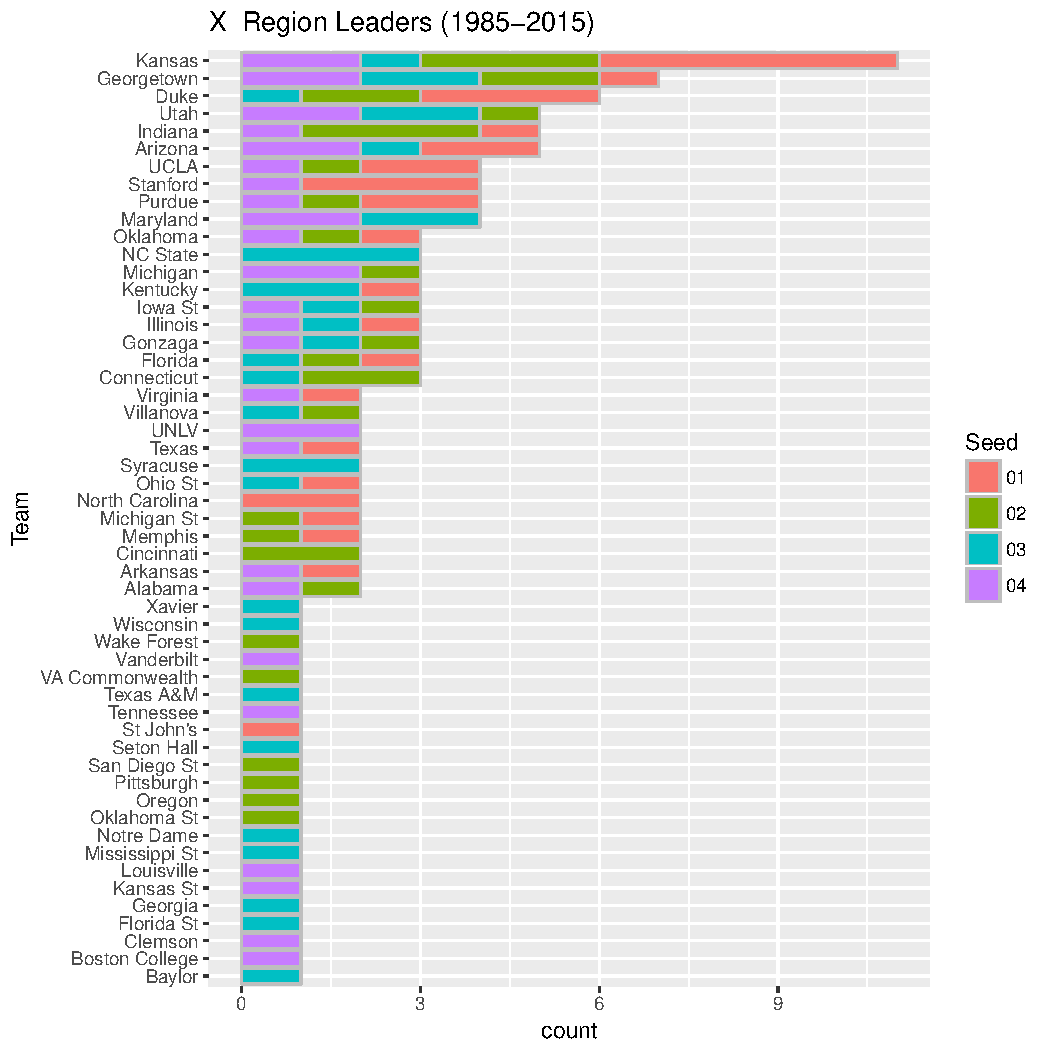
\includegraphics[]{455Project/XConfLeader.pdf}
	\caption[leaders]{Best teams in the X Region by reporting the teams only entering within the top 4 seeds from the years 1985-2015. We see that teams that get the number one seed tend to stay within the top four }
	\label{rVals}
\end{figure}
To specify, the "X" conference is a region up to change with each season. In general, X is usually the West, Midwest, Southeast, or the South. "W" almost always represents the East, and so on for Y and Z. 
\begin{figure}[H]
	\centering
	\includegraphics[]{455Project/overLeaders.pdf}
	\caption[overallLeaders]{Best teams over all regions. This shows the upper echelon of basketball teams and the many others that try and compete}
	\label{rVals}
\end{figure}
We can also look at how these teams tend to actually preform in the tournaments by seeing how many games they have played over all these years.
\begin{figure}[H]
	\centering
	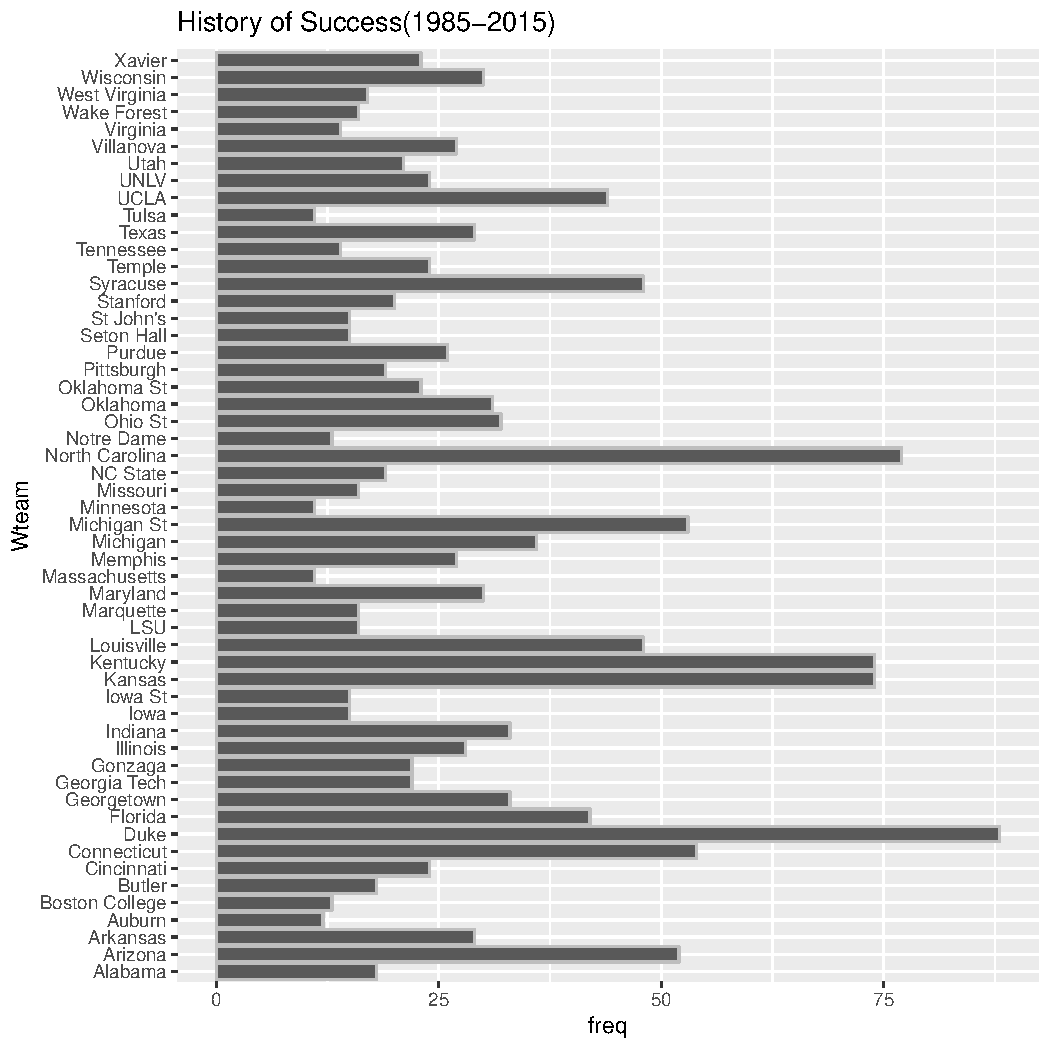
\includegraphics[]{455Project/HistOfSuccess2.pdf}
	\caption[HistOfSuccess]{This shows the teams with the most appearances in the march madness tournament. The more appearances illustrate they make it further in the tournament than others}
	\label{rVals}
\end{figure}

Overall, this is to show that the parameters of $\beta_s$, or seed, and $\beta_a$, appearances, of a teams history is indicative of their future success.
\section*{Proposed Model}

\end{document}
